\documentclass{article}

\usepackage{graphicx}
%\usepackage{geometry}
\usepackage{placeins} % use float barriers
\usepackage{float}
\usepackage{subcaption}
\usepackage{longtable}
\usepackage[a4paper,margin=1in]{geometry}
\usepackage{grffile}
\usepackage{multirow}

\title{RL benchmark for the reaching task}
\date{}

\begin{document}

\maketitle


\section{Raw results}


% Please add the following required packages to your document preamble:
% \usepackage{multirow}
%\begin{table}[]
\begin{longtable}{llllll} \hline
Environment                                                                     & Physics engine                                                           & RL algorithm & Train time (min) {[}1{]} & Success ratio {[}2{]} & Average reach time {[}3{]}  \\ \hline
\multirow{8}{*}{\begin{tabular}[c]{@{}l@{}}Reacher 2D\\ 1 joint\end{tabular}}   & \multirow{8}{*}{PyBullet}                                                & A2C          & 10.83                    & 0.14                  & 32.36                      \\
                                                                                &                                                                          & ACKTR        & 8.98                     & 0.16                  & 33.94                      \\
                                                                                &                                                                          & DDPG         & 31.63                    & 0.07                  & 14                         \\
                                                                                &                                                                          & PPO1         & 9.01                     & 0.17                  & 17.18                      \\
                                                                                &                                                                          & PPO2         & 9.57                     & 0.09                  & 8.56                       \\
                                                                                &                                                                          & SAC          & 49.41                    & 0.13                  & 13.85                      \\
                                                                                &                                                                          & TRPO         & 7.79                     & 0.12                  & 35.42                      \\
                                                                                &                                                                          & TD3          & 32.42                    & 0.1                   & 21.9                       \\ \hline
\multirow{8}{*}{\begin{tabular}[c]{@{}l@{}}Reacher 2D \\ 2 joints\end{tabular}} & \multirow{8}{*}{PyBullet}                                                & A2C          & 12.13                    & 0.15                  & 39.6                       \\
                                                                                &                                                                          & ACKTR        & 9.83                     & 0.91                  & 42.73                      \\
                                                                                &                                                                          & DDPG         & 32.68                    & 0.08                  & 18.75                      \\
                                                                                &                                                                          & PPO1         & 9.8                      & 0.04                  & 23                         \\
                                                                                &                                                                          & PPO2         & 10.18                    & 0.09                  & 35.89                      \\
                                                                                &                                                                          & SAC          & 45.35                    & 0.5                   & 28.59                      \\
                                                                                &                                                                          & TRPO         & 8.59                     & 0.01                  & 84                         \\
                                                                                &                                                                          & TD3          & 33.29                    & 0.33                  & 40.64                      \\ \hline
\multirow{8}{*}{\begin{tabular}[c]{@{}l@{}}Reacher 2D\\ 3 joints\end{tabular}}  & \multirow{8}{*}{PyBullet}                                                & A2C          & 12.34                    & 0.14                  & 41                         \\
                                                                                &                                                                          & ACKTR        & 10.44                    & 0.59                  & 58.35                      \\
                                                                                &                                                                          & DDPG         & 33.61                    & 0.12                  & 34.17                      \\
                                                                                &                                                                          & PPO1         & 10.34                    & 0.09                  & 55.22                      \\
                                                                                &                                                                          & PPO2         & 10.77                    & 0.12                  & 42.58                      \\
                                                                                &                                                                          & SAC          & 45.61                    & 0.36                  & 49.03                      \\
                                                                                &                                                                          & TRPO         & 9.09                     & 0.14                  & 54.93                      \\
                                                                                &                                                                          & TD3          & 34.13                    & 0.13                  & 36.54                      \\ \hline
\multirow{8}{*}{\begin{tabular}[c]{@{}l@{}}Reacher 2D\\ 4 joints\end{tabular}}  & \multirow{8}{*}{PyBullet}                                                & A2C          & 12.84                    & 0.06                  & 43.67                      \\
                                                                                &                                                                          & ACKTR        & 10.93                    & 0.13                  & 49.46                      \\
                                                                                &                                                                          & DDPG         & 34.51                    & 0.08                  & 57.25                      \\
                                                                                &                                                                          & PPO1         & 10.96                    & 0.08                  & 26.12                      \\
                                                                                &                                                                          & PPO2         & 11.25                    & 0.07                  & 45.43                      \\
                                                                                &                                                                          & SAC          & 46.8                     & 0.27                  & 45.15                      \\
                                                                                &                                                                          & TRPO         & 9.61                     & 0.13                  & 56.54                      \\
                                                                                &                                                                          & TD3          & 34.59                    & 0.21                  & 45.38                      \\ \hline
\multirow{8}{*}{\begin{tabular}[c]{@{}l@{}}Reacher 2D\\ 5 joints\end{tabular}}  & \multirow{8}{*}{PyBullet}                                                & A2C          & 13.43                    & 0.12                  & 49.17                      \\
                                                                                &                                                                          & ACKTR        & 11.46                    & 0.17                  & 74.65                      \\
                                                                                &                                                                          & DDPG         & 34.73                    & 0.04                  & 32.5                       \\
                                                                                &                                                                          & PPO1         & 11.49                    & 0.07                  & 43.43                      \\
                                                                                &                                                                          & PPO2         & 11.85                    & 0.05                  & 55.8                       \\
                                                                                &                                                                          & SAC          & 47.11                    & 0.22                  & 49.86                      \\
                                                                                &                                                                          & TRPO         & 10.16                    & 0.06                  & 62.67                      \\
                                                                                &                                                                          & TD3          & 36.76                    & 0.18                  & 49.22                      \\ \hline
\multirow{8}{*}{\begin{tabular}[c]{@{}l@{}}Reacher 2D\\ 6 joints\end{tabular}}  & \multirow{8}{*}{PyBullet}                                                & A2C          & 14.47                    & 0.04                  & 60.25                      \\
                                                                                &                                                                          & ACKTR        & 12.38                    & 0.14                  & 67.86                      \\
                                                                                &                                                                          & DDPG         & 35.98                    & 0.11                  & 49.82                      \\
                                                                                &                                                                          & PPO1         & 12.39                    & 0.05                  & 48                         \\
                                                                                &                                                                          & PPO2         & 12.61                    & 0.07                  & 30.71                      \\
                                                                                &                                                                          & SAC          & 46.19                    & 0.14                  & 45.93                      \\
                                                                                &                                                                          & TRPO         & 10.63                    & 0.06                  & 34.67                      \\
                                                                                &                                                                          & TD3          & 35.74                    & 0.07                  & 58.14                      \\ \hline
\multirow{8}{*}{\begin{tabular}[c]{@{}l@{}}Jaco 3D\\ 6 joints\end{tabular}}     & \multirow{8}{*}{\begin{tabular}[c]{@{}l@{}}ROS / \\ Gazebo\end{tabular}} & A2C          &                          &                       &                            \\
                                                                                &                                                                          & ACKTR        &                          &                       &                            \\
                                                                                &                                                                          & DDPG         &                          &                       &                            \\
                                                                                &                                                                          & PPO1         &                          &                       &                            \\
                                                                                &                                                                          & PPO2         &                          &                       &                            \\
                                                                                &                                                                          & SAC          &                          &                       &                            \\
                                                                                &                                                                          & TRPO         &                          &                       &                            \\
                                                                                &                                                                          & TD3          &                          &                       &                            \\ \hline
\multirow{8}{*}{\begin{tabular}[c]{@{}l@{}}Jaco 3D\\ 6 joints\end{tabular}}     & \multirow{8}{*}{Real world}                                              & A2C          &                          &                       &                            \\
                                                                                &                                                                          & ACKTR        &                          &                       &                            \\
                                                                                &                                                                          & DDPG         &                          &                       &                            \\
                                                                                &                                                                          & PPO1         &                          &                       &                            \\
                                                                                &                                                                          & PPO2         &                          &                       &                            \\
                                                                                &                                                                          & SAC          &                          &                       &                            \\
                                                                                &                                                                          & TRPO         &                          &                       &                            \\
                                                                                &                                                                          & TD3          &                          &                       &                         \\  
\hline
\end{longtable}
%\end{table}


[1] Train time (min) : Wall time to train for 1M time steps. \\ 

[2] Success ratio: number of successful episodes / number of reachable episodes (in this case: number of reachable episodes = 100) \\ 
An episode is successful if the distance between the finger tip and the target is less or equal to 0.01. \\ 
The length of a robot link is 0.1.

[3] Average reaching time : sum (number of time steps of all successful episodes) /  number of successful episodes \\ 
An episode has a maximum of 100 time steps. \\ 

The RL algorithm used here are from the Stable baselines baselines implementation using the default parameters. \\ 



Complexity to add later:
\begin{enumerate}
  \item Reach target position and orientation
  \item Presence of obstacles
  \item Target is moving during operation
\end{enumerate}

\section{Performance plots - sorted by algorithm}


\begin{figure}[H]
    \centering
    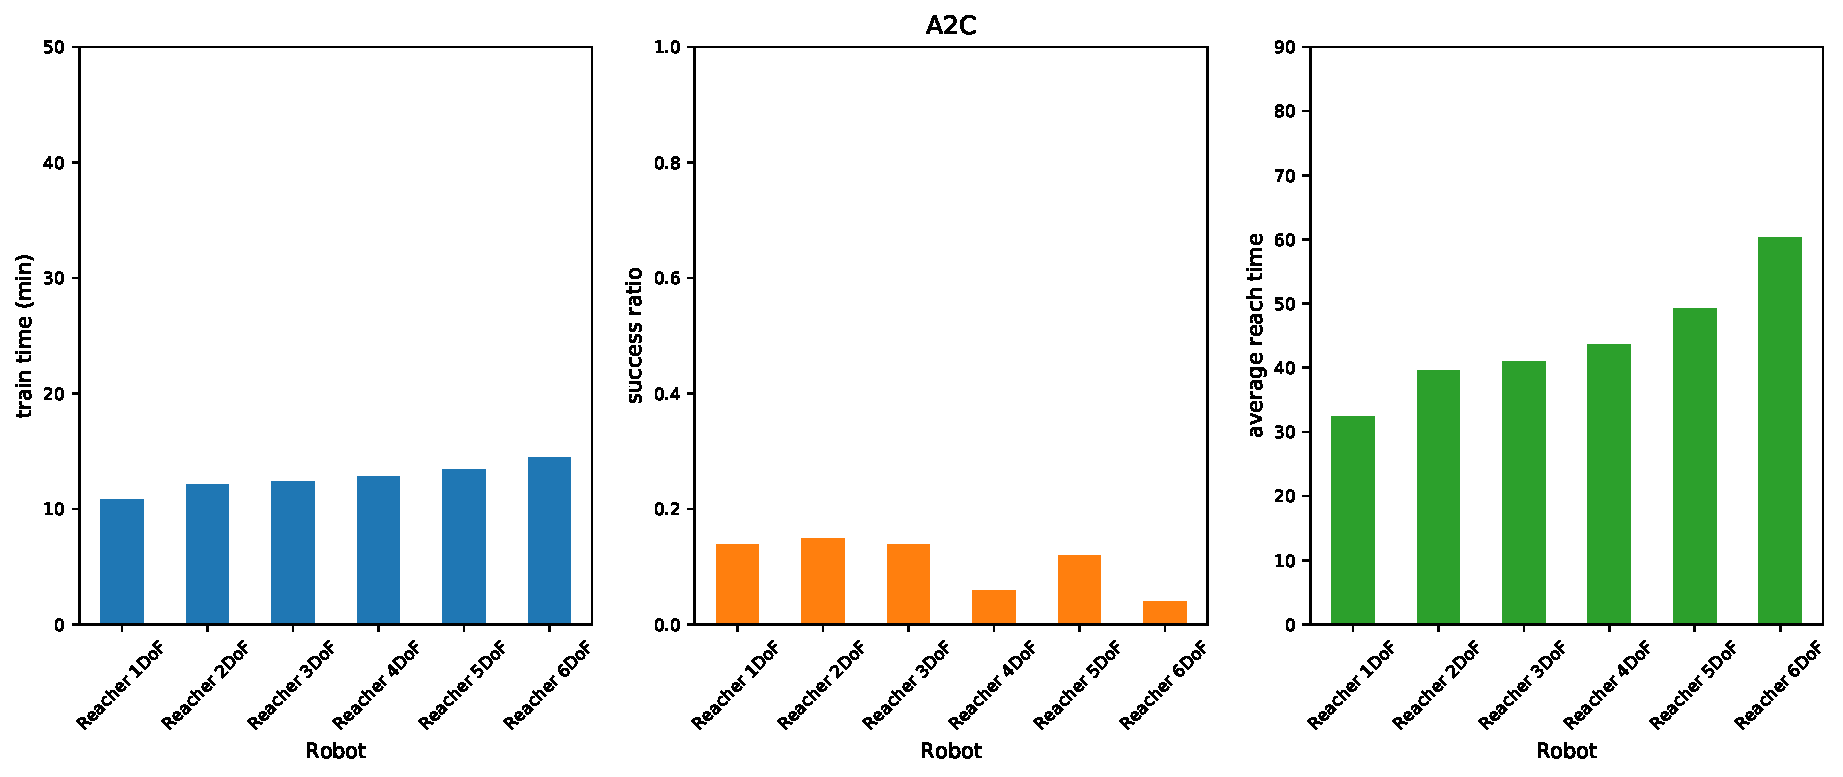
\includegraphics[width=\textwidth]{../A2C.pdf}
\caption{Performance metrics of the A2C algorithm.}
\end{figure}

\begin{figure}[H]
    \centering
    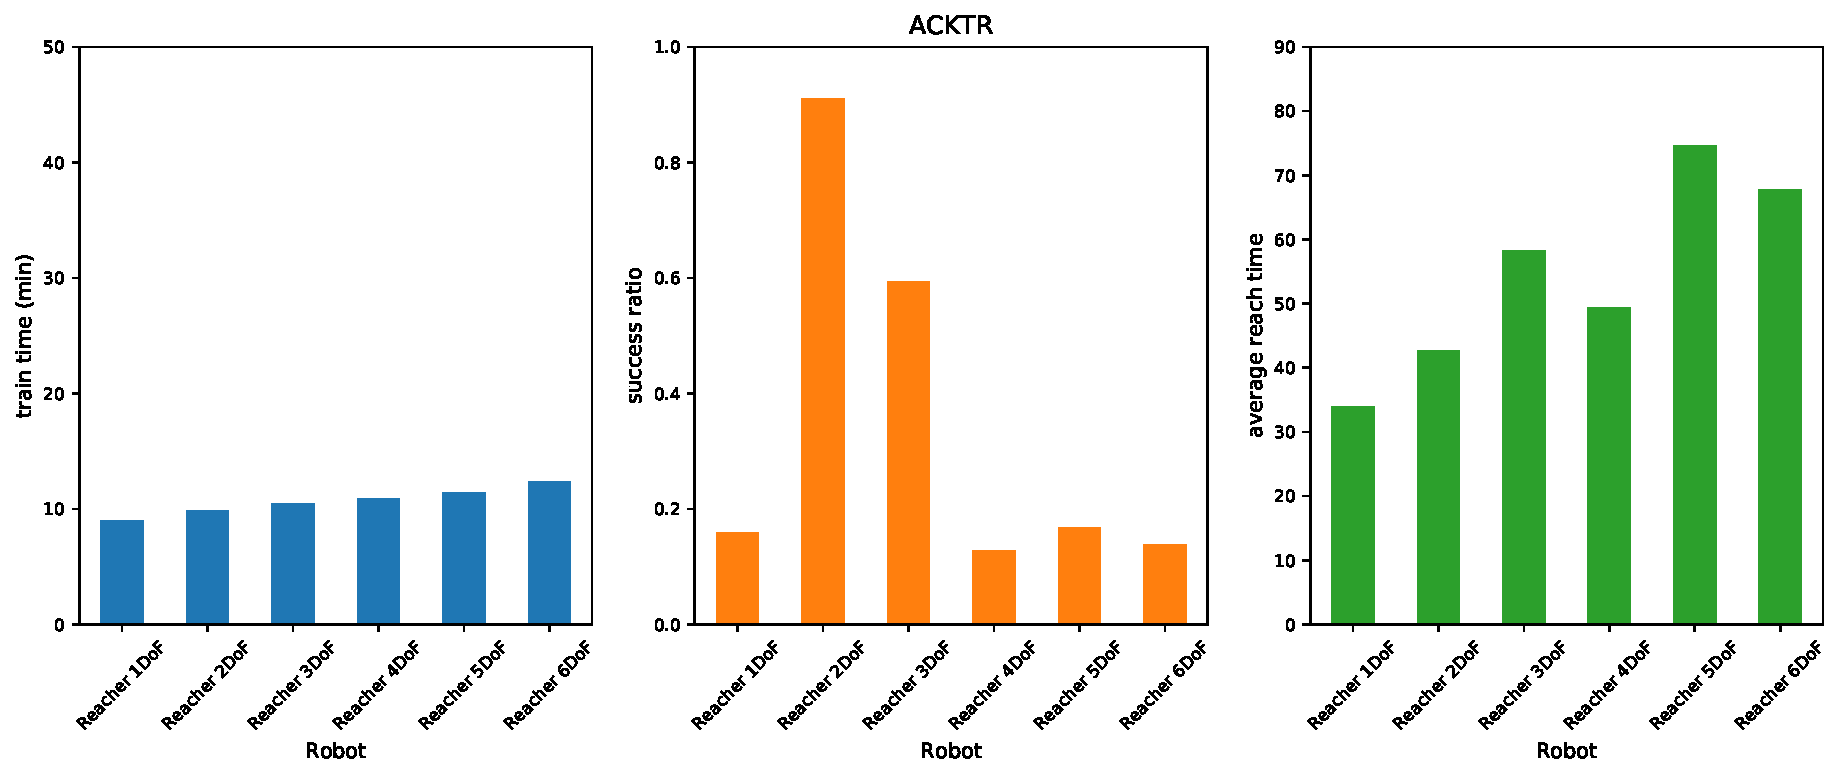
\includegraphics[width=\textwidth]{../ACKTR.pdf}
\caption{Performance metrics of the ACKTR algorithm.}
\end{figure}

\begin{figure}[H]
    \centering
    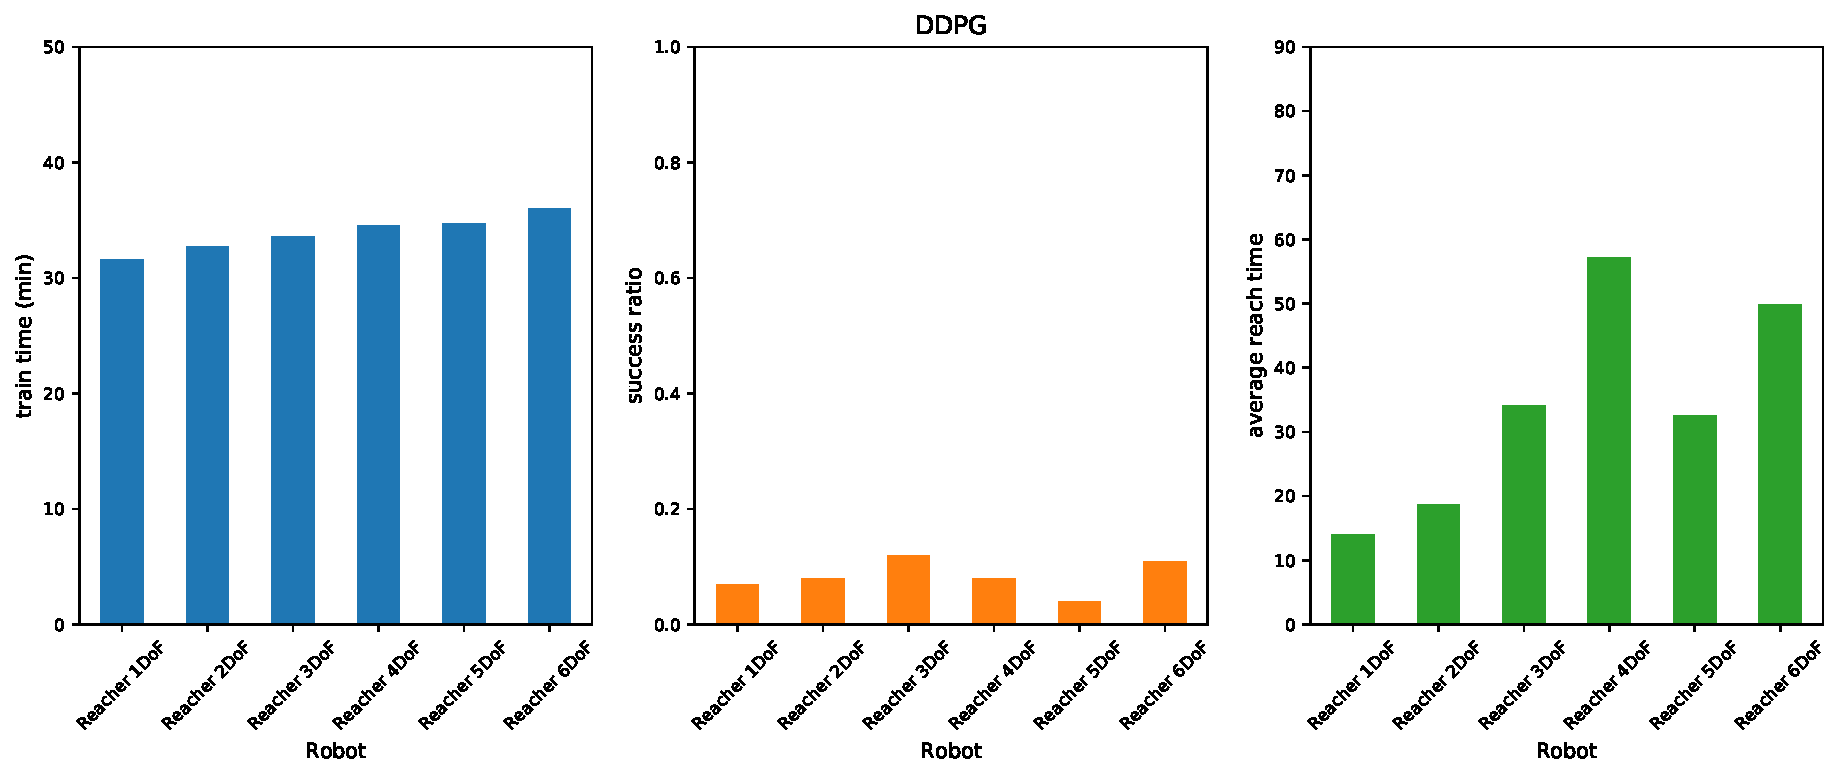
\includegraphics[width=\textwidth]{../DDPG.pdf}
\caption{Performance metrics of the DDPG algorithm.}
\end{figure}

\begin{figure}[H]
    \centering
    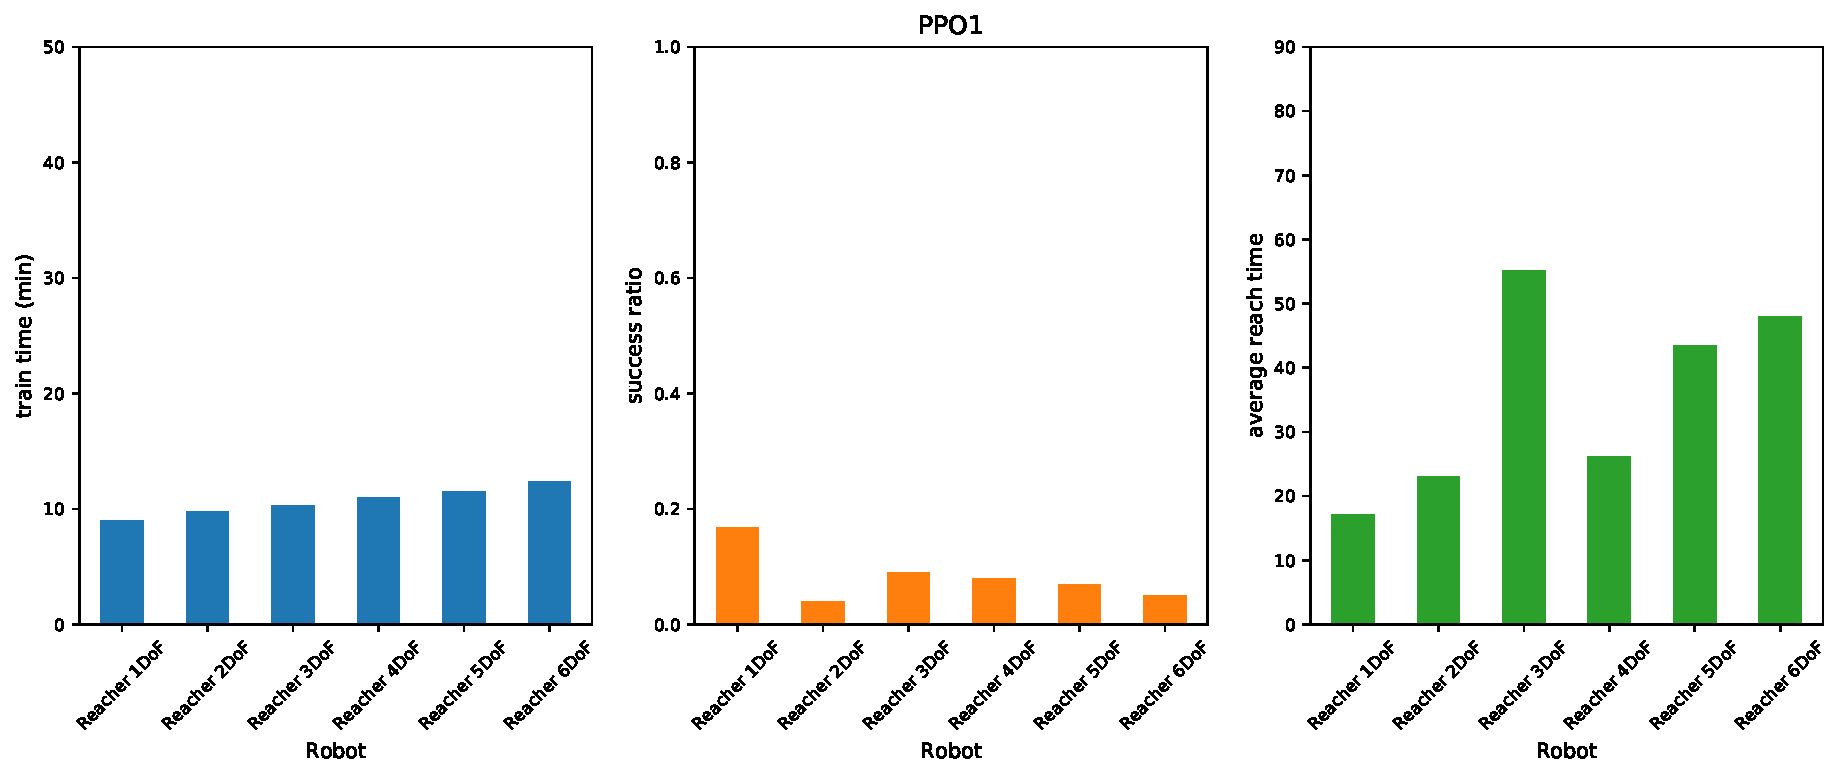
\includegraphics[width=\textwidth]{../PPO1.pdf}
\caption{Performance metrics of the PPO1 algorithm.}
\end{figure}

\begin{figure}[H]
    \centering
    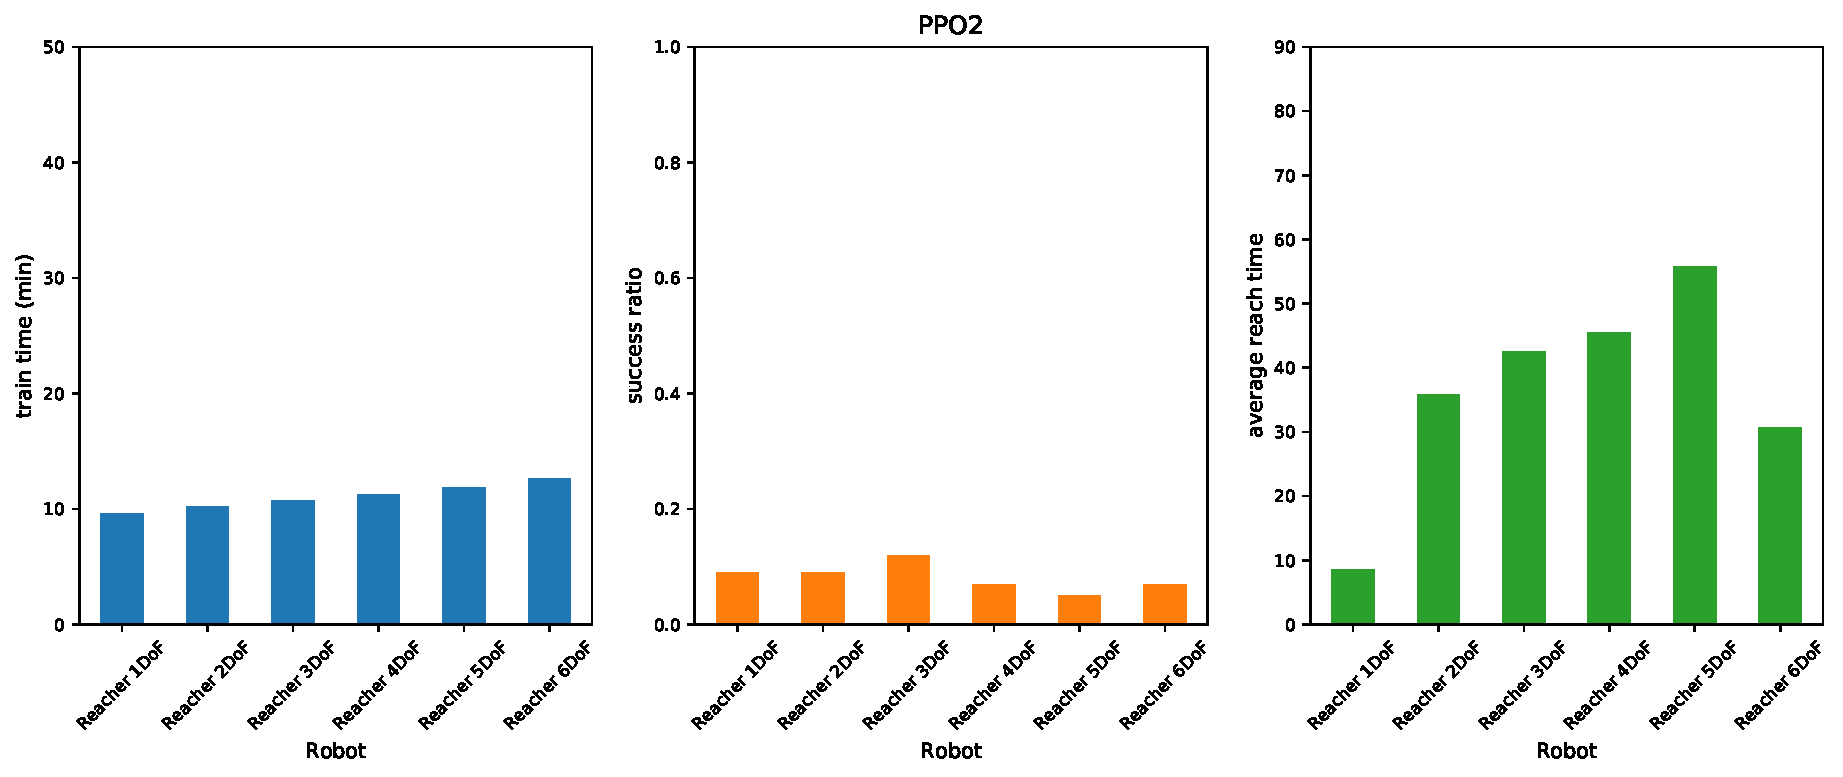
\includegraphics[width=\textwidth]{../PPO2.pdf}
\caption{Performance metrics of the PPO2 algorithm.}
\end{figure}

\begin{figure}[H]
    \centering
    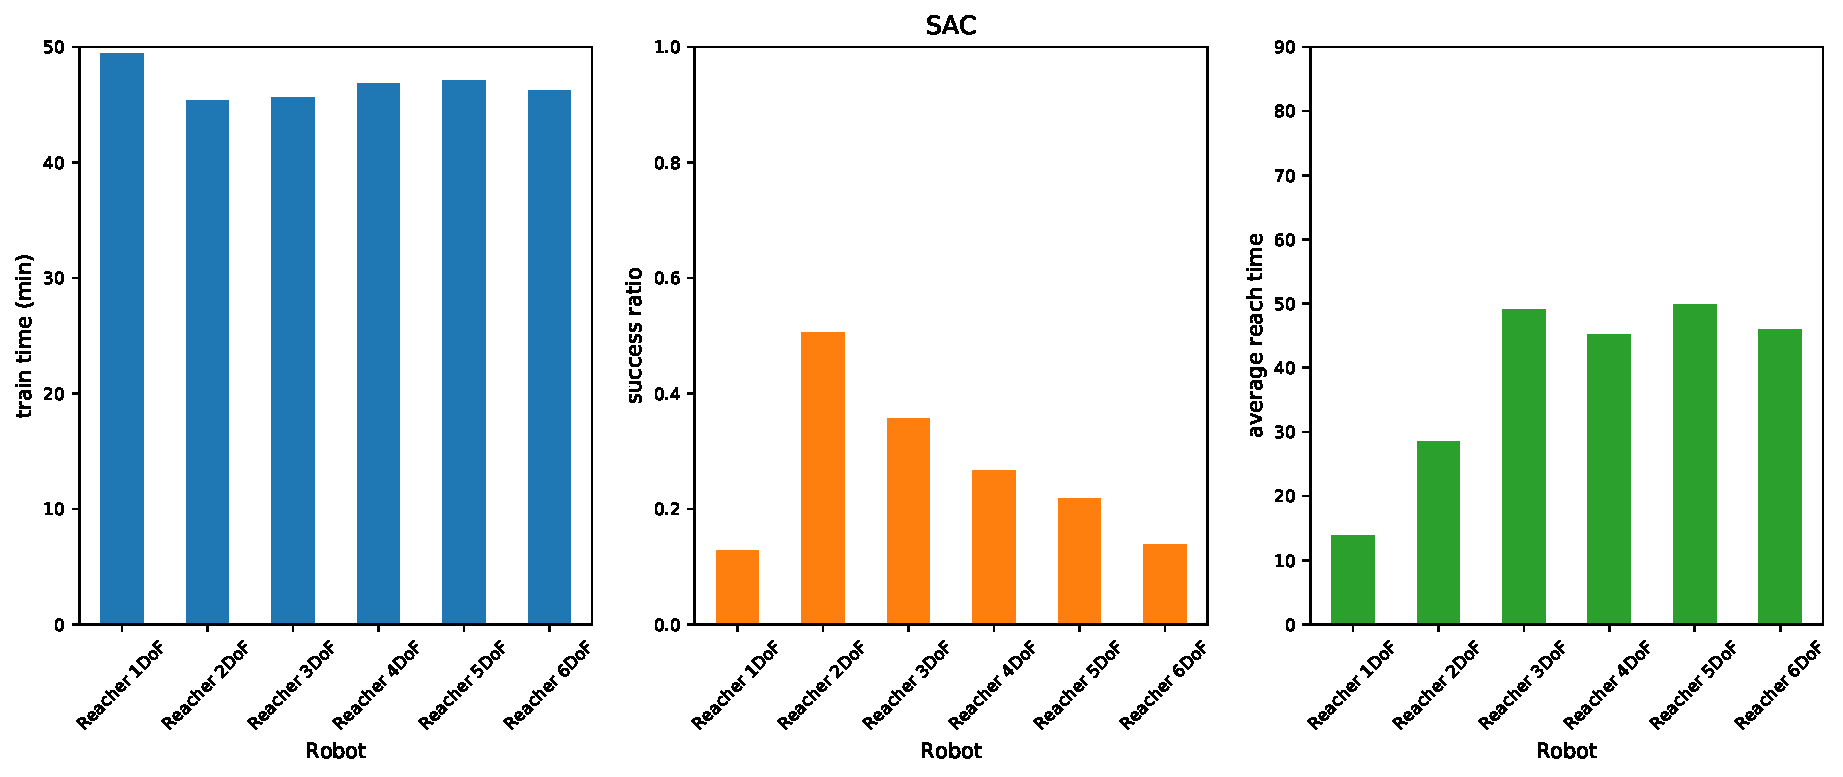
\includegraphics[width=\textwidth]{../SAC.pdf}
\caption{Performance metrics of the SAC algorithm.}
\end{figure}

\begin{figure}[H]
    \centering
    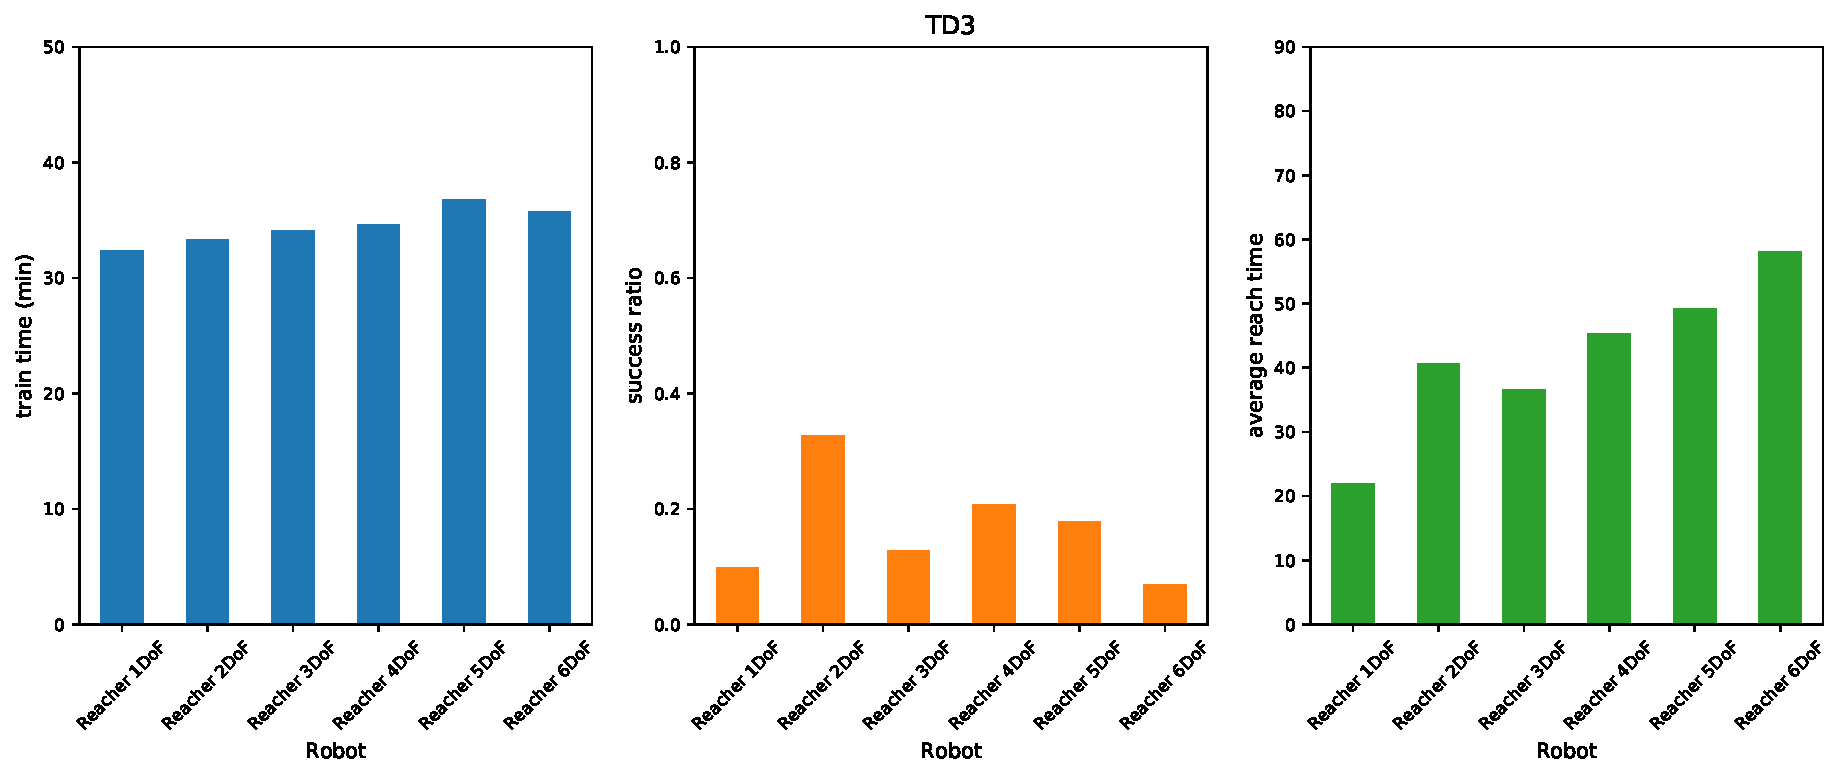
\includegraphics[width=\textwidth]{../TD3.pdf}
\caption{Performance metrics of the TD3 algorithm.}
\end{figure}

\begin{figure}[H]
    \centering
    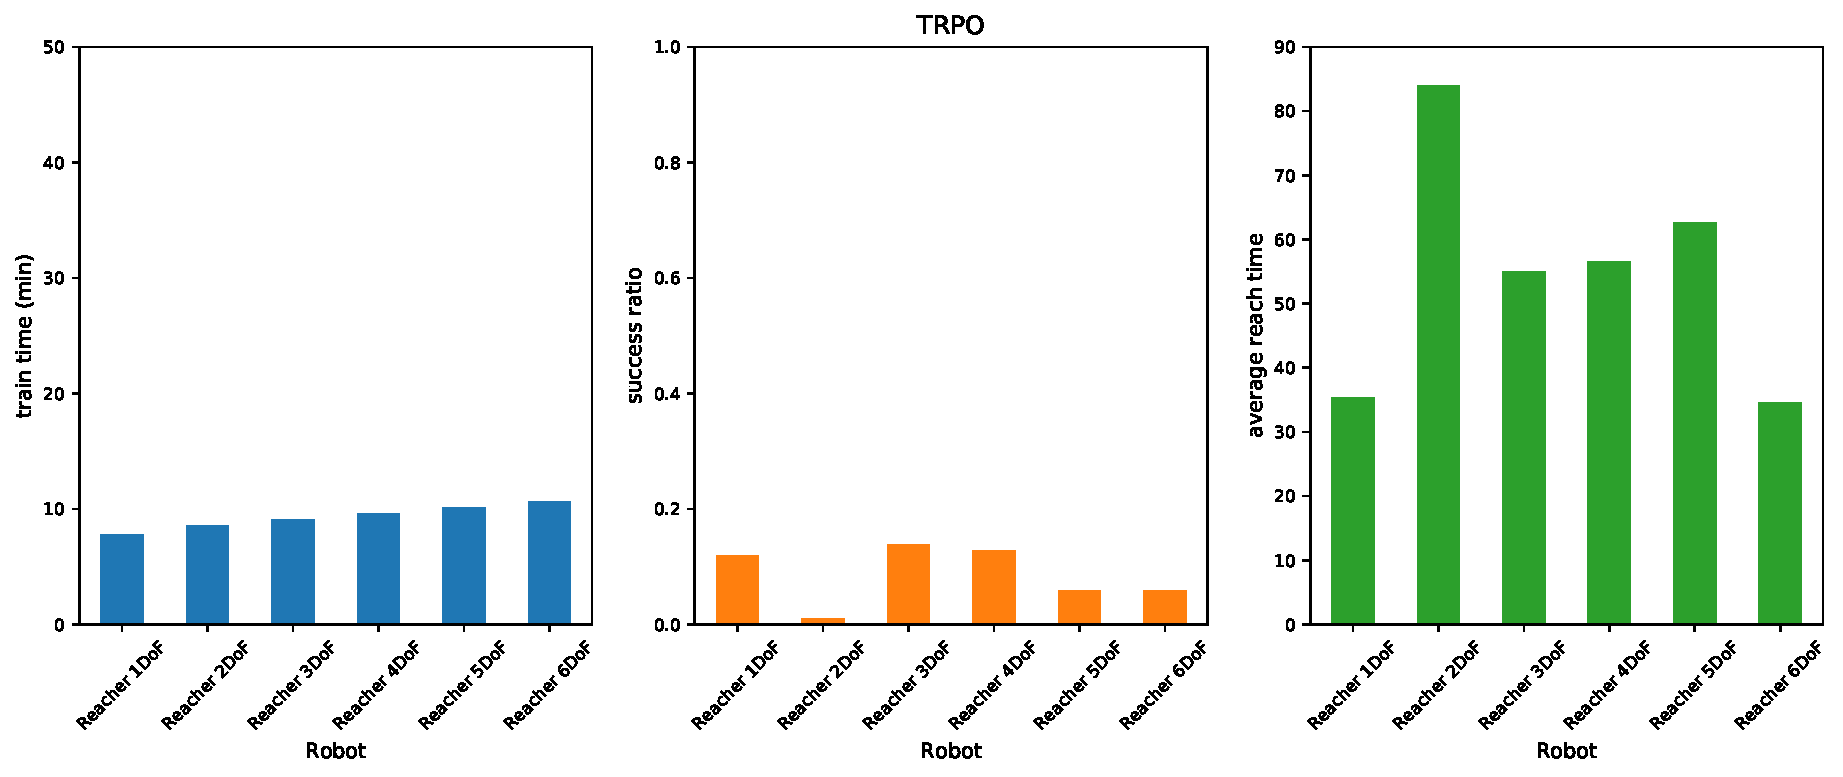
\includegraphics[width=\textwidth]{../TRPO.pdf}
\caption{Performance metrics of the TRPO algorithm.}
\end{figure}



\section{Performance plots - sorted by number of joints}

\begin{figure}[H]
    \centering
    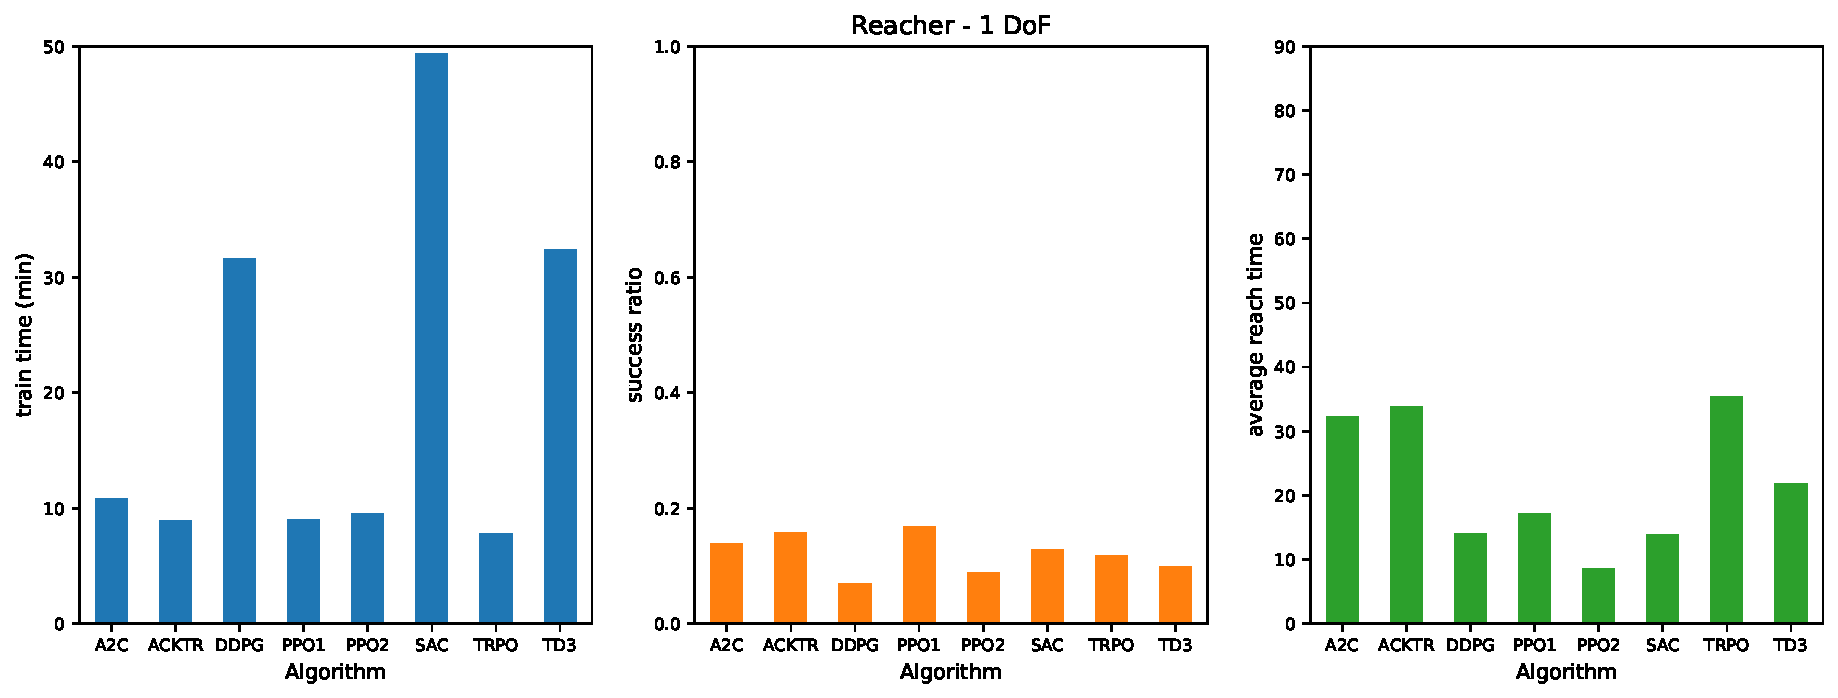
\includegraphics[width=\textwidth]{../Reacher1Dof-v0/reacher1.pdf}
\caption{Performance metrics of the Reacher 1 DoF robot.}
\end{figure}

\begin{figure}[H]
    \centering
    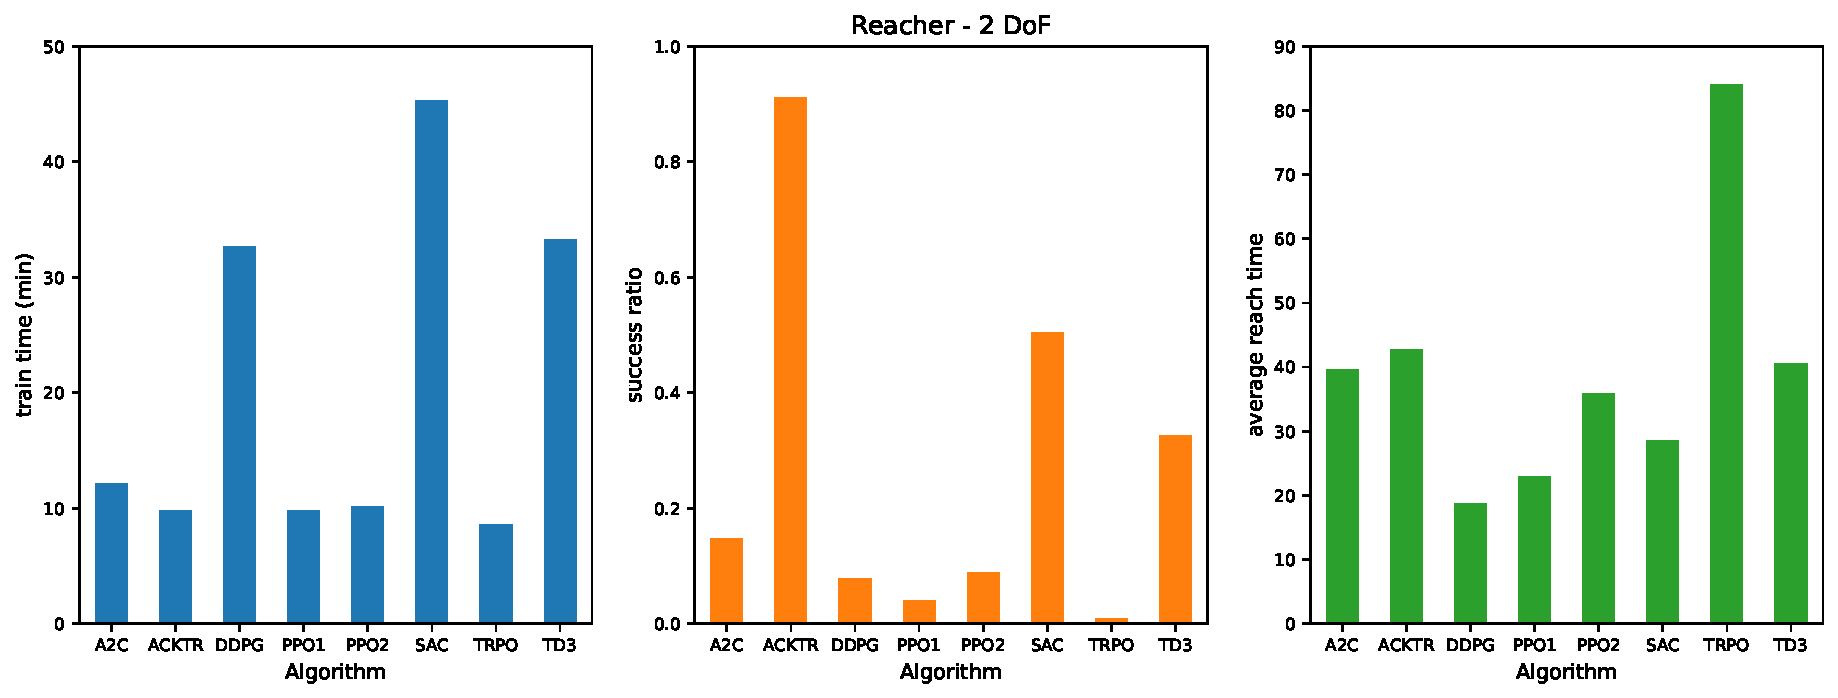
\includegraphics[width=\textwidth]{../Reacher2Dof-v0/reacher2.pdf}
\caption{Performance metrics of the Reacher 2 DoF robot.}
\end{figure}

\begin{figure}[H]
    \centering
    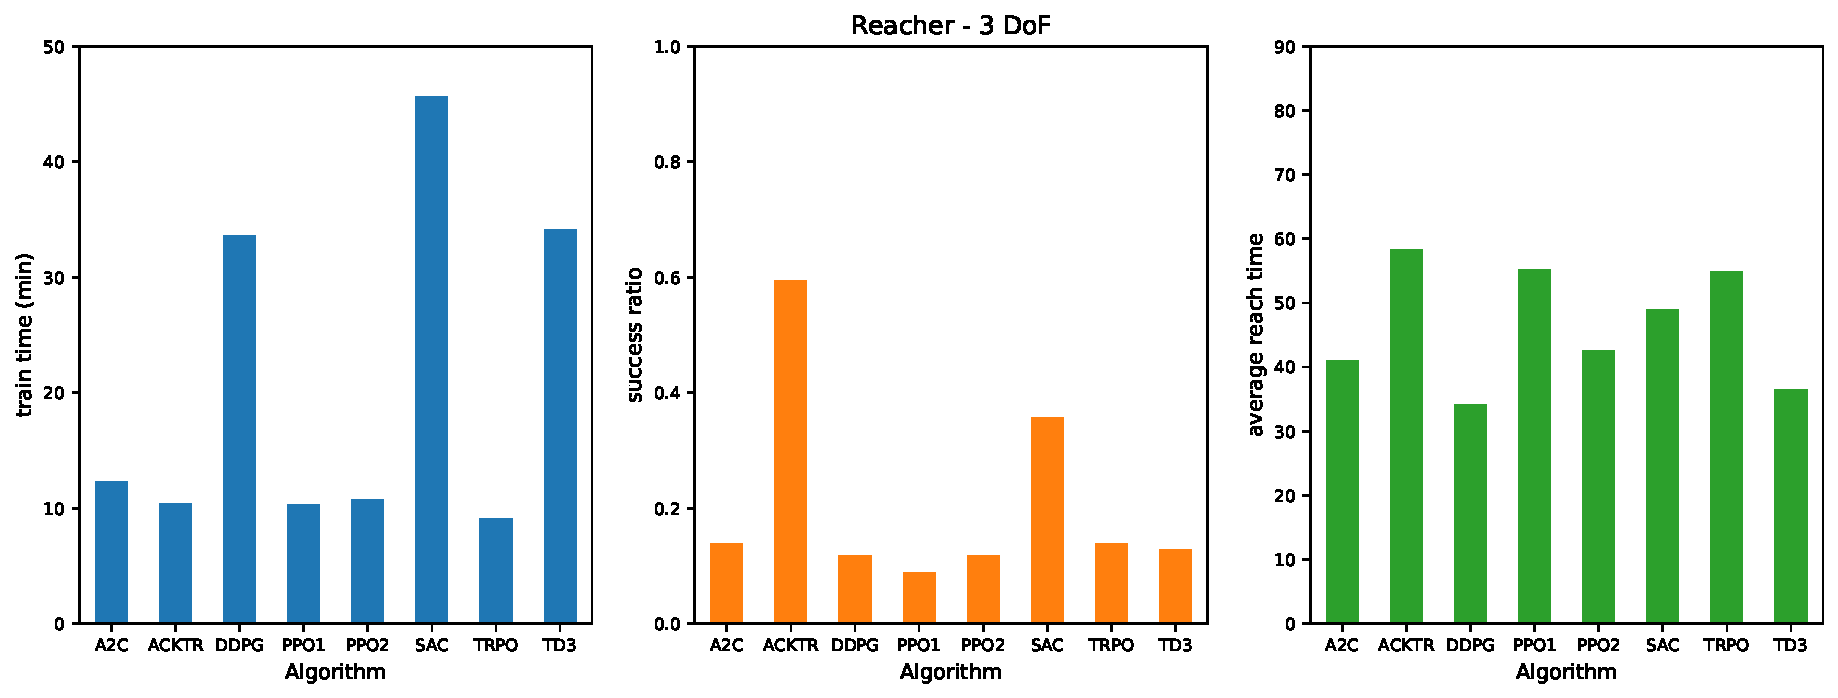
\includegraphics[width=\textwidth]{../Reacher3Dof-v0/reacher3.pdf}
\caption{Performance metrics of the Reacher 3 DoF robot.}
\end{figure}

\begin{figure}[H]
    \centering
    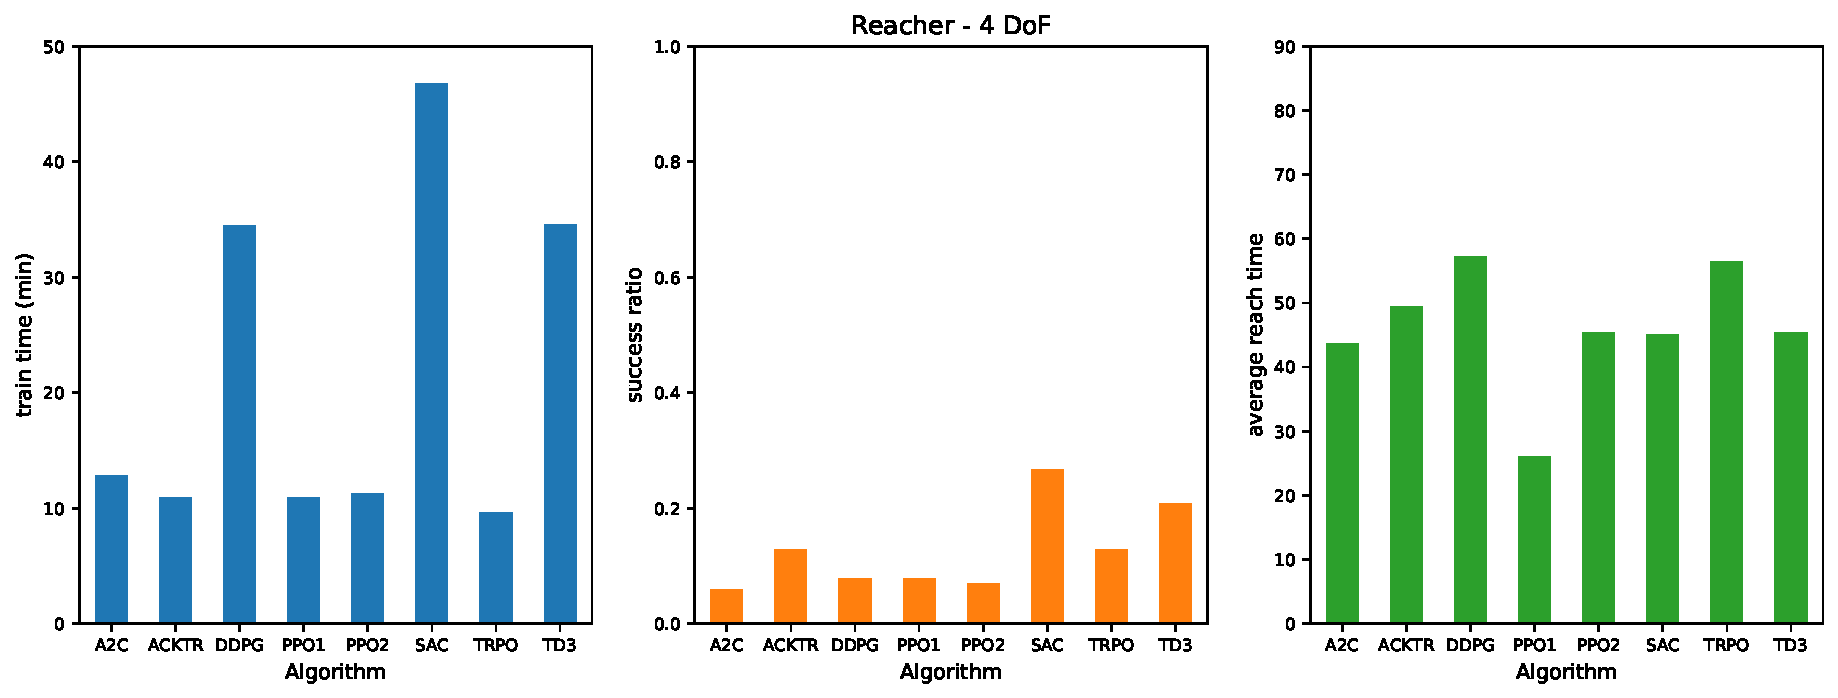
\includegraphics[width=\textwidth]{../Reacher4Dof-v0/reacher4.pdf}
\caption{Performance metrics of the Reacher 4 DoF robot.}
\end{figure}

\begin{figure}[H]
    \centering
    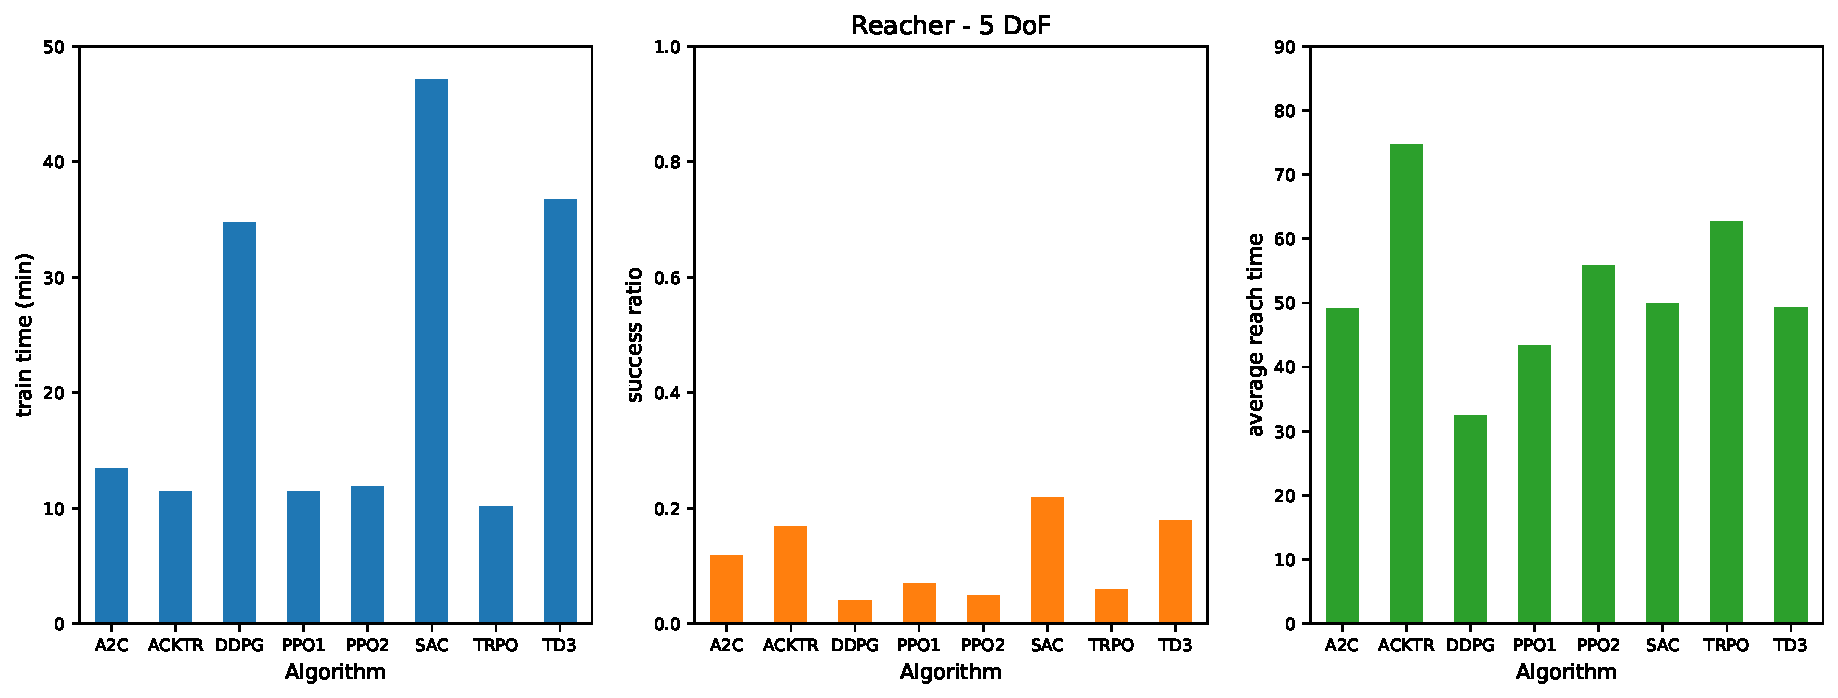
\includegraphics[width=\textwidth]{../Reacher5Dof-v0/reacher5.pdf}
\caption{Performance metrics of the Reacher 5 DoF robot.}
\end{figure}

\begin{figure}[H]
    \centering
    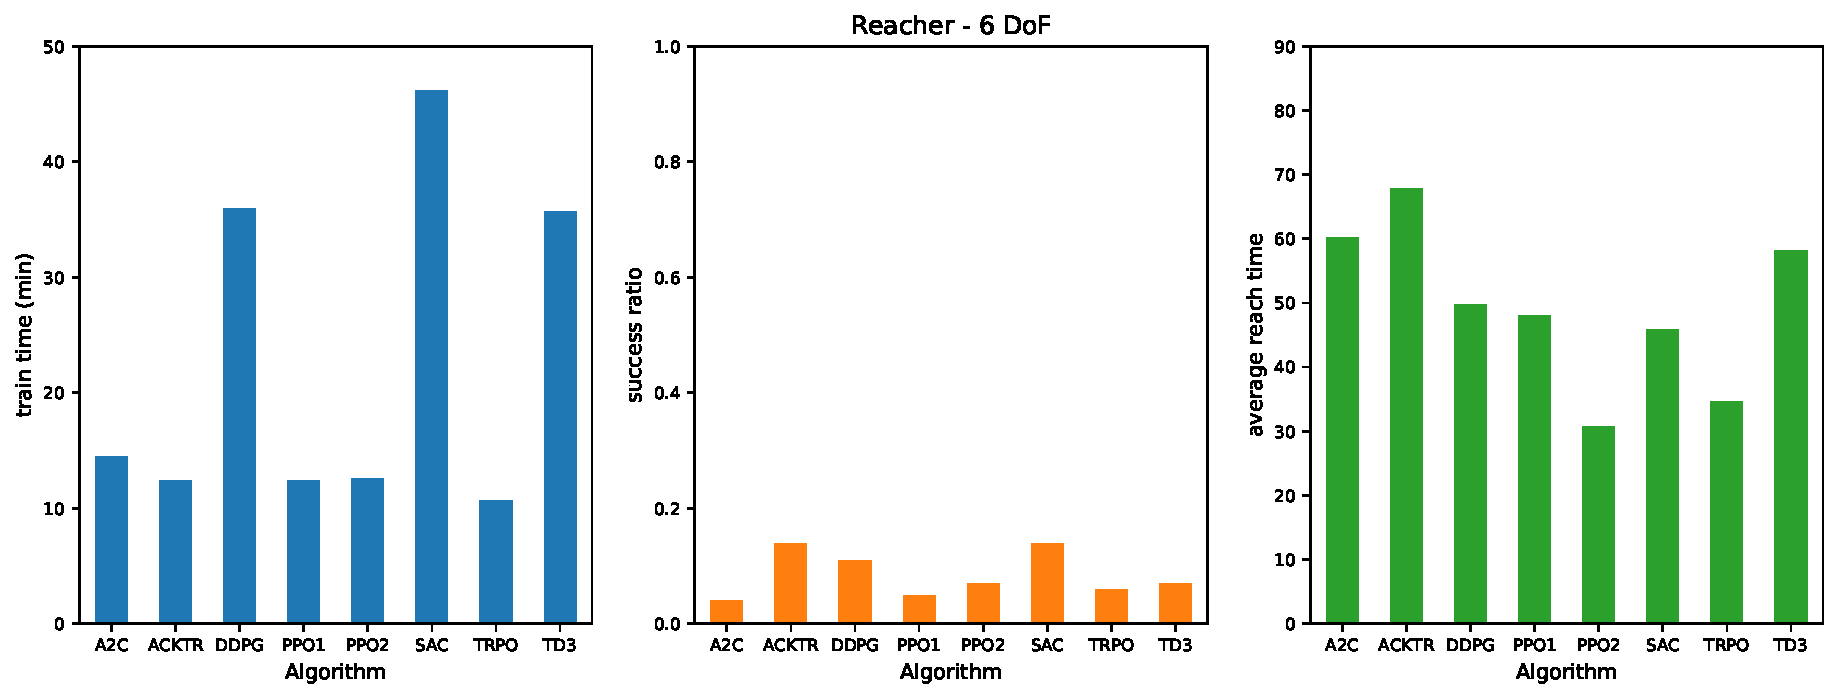
\includegraphics[width=\textwidth]{../Reacher6Dof-v0/reacher6.pdf}
\caption{Performance metrics of the Reacher 6 DoF robot.}
\end{figure}


%
%
%\section{Continous recording: OK}
%
%1h of data = 11 MB \\
%approx 100 GB for 1 year of data
%
%
%\section{CSklearn classification}
%
%\begin{longtable}
%
%
%
%
%
%\begin{enumerate}
%  \item Reformat training data to match format from DAQ
%  \item Extract features
%  \item Impute NaNs
%  \item Train test split
%  \item Iterate over decomposition and classifiers
%  \begin{enumerate}
%     \item Build pipeline object: standardscaler > decomposition > (minmaxscaler) > classifier
%     \item Fit model
%     \item Calculate train, test and cross-validation accuracy   
%     \item Plot decision boundary
%  \end{enumerate}  
%  \item Select best model and save the trained model as a binary
%  \item Classify real-time incoming data using the trained model
%  
%\end{enumerate}
%
%\subsection{Standard scaler + Decomposition + Classifier}
%
%
%\begin{figure}[H]
%\centering
%\begin{subfigure}{0.49\textwidth}
%  \centering
%  \includegraphics[width=\textwidth]{../../Data_and_plots/tests_19.11.25-26/plots/11_dim_red_real_time/std_dec_clf/best/IncrementalPCA_BaggingClassifier_xval_93.78_test_100.0_train_100.0.png} 
%
%\end{subfigure}
%\begin{subfigure}{0.49\textwidth}
%  \centering
%  \includegraphics[width=\textwidth]{../../Data_and_plots/tests_19.11.25-26/plots/11_dim_red_real_time/std_dec_clf/best/IncrementalPCA_GaussianNB_xval_93.94_test_89.56_train_97.06.png} 
%
%\end{subfigure}
%\end{figure}
%
%
%\begin{figure}[H]
%\centering
%\begin{subfigure}{0.49\textwidth}
%  \centering
%  \includegraphics[width=\textwidth]{../../Data_and_plots/tests_19.11.25-26/plots/11_dim_red_real_time/std_dec_clf/best/IncrementalPCA_RandomForestClassifier_xval_93.78_test_100.0_train_100.0.png} 
%
%\end{subfigure}
%\begin{subfigure}{0.49\textwidth}
%  \centering
%  \includegraphics[width=\textwidth]{../../Data_and_plots/tests_19.11.25-26/plots/11_dim_red_real_time/std_dec_clf/best/KernelPCA_DecisionTreeClassifier_xval_93.78_test_89.56_train_100.0.png} 
%
%\end{subfigure}
%\end{figure}
%
%\begin{figure}[H]
%\centering
%\begin{subfigure}{0.49\textwidth}
%  \centering
%  \includegraphics[width=\textwidth]{../../Data_and_plots/tests_19.11.25-26/plots/11_dim_red_real_time/std_dec_clf/best/KernelPCA_GaussianNB_xval_93.94_test_89.56_train_97.06.png} 
%
%\end{subfigure}
%\begin{subfigure}{0.49\textwidth}
%  \centering
%  \includegraphics[width=\textwidth]{../../Data_and_plots/tests_19.11.25-26/plots/11_dim_red_real_time/std_dec_clf/best/NMF_ExtraTreeClassifier_xval_94.64_test_89.56_train_100.0.png} 
%
%\end{subfigure}
%\end{figure}
%
%\begin{figure}[H]
%\centering
%\begin{subfigure}{0.49\textwidth}
%  \centering
%  \includegraphics[width=\textwidth]{../../Data_and_plots/tests_19.11.25-26/plots/11_dim_red_real_time/std_dec_clf/best/PCA_DecisionTreeClassifier_xval_93.78_test_89.56_train_100.0.png} 
%
%\end{subfigure}
%\begin{subfigure}{0.49\textwidth}
%  \centering
%  \includegraphics[width=\textwidth]{../../Data_and_plots/tests_19.11.25-26/plots/11_dim_red_real_time/std_dec_clf/best/PCA_GaussianNB_xval_93.94_test_89.56_train_97.06.png} 
%
%\end{subfigure}
%\end{figure}
%
%\begin{figure}[H]
%\centering
%\begin{subfigure}{0.49\textwidth}
%  \centering
%  \includegraphics[width=\textwidth]{../../Data_and_plots/tests_19.11.25-26/plots/11_dim_red_real_time/std_dec_clf/best/PCA_GaussianProcessClassifier_xval_85.0_test_100.0_train_100.0.png} 
%
%\end{subfigure}
%\begin{subfigure}{0.49\textwidth}
%  \centering
%  \includegraphics[width=\textwidth]{../../Data_and_plots/tests_19.11.25-26/plots/11_dim_red_real_time/std_dec_clf/best/TruncatedSVD_GaussianNB_xval_94.43_test_100.0_train_94.07.png} 
%
%\end{subfigure}
%\end{figure}
%
%
%
%\begin{table}[H]
%\begin{tabular}{lllll}
%\textbf{decomposition} & \textbf{algorithm}         & \textbf{cross-validation} & \textbf{training accuracy} & \textbf{test accuracy} \\ \hline
%NMF                    & ExtraTreeClassifier        & 94.64                     & 100                        & 89.56                  \\
%TruncatedSVD           & GaussianNB                 & 94.43                     & 94.07                      & 100                    \\
%PCA                    & GaussianNB                 & 93.94                     & 97.06                      & 89.56                  \\
%KernelPCA              & GaussianNB                 & 93.94                     & 97.06                      & 89.56                  \\
%IncrementalPCA         & GaussianNB                 & 93.94                     & 97.06                      & 89.56                  \\
%IncrementalPCA         & BaggingClassifier          & 93.78                     & 100                        & 100                    \\
%KernelPCA              & DecisionTreeClassifier     & 93.78                     & 100                        & 89.56                  \\
%PCA                    & DecisionTreeClassifier     & 93.78                     & 100                        & 89.56                  \\
%IncrementalPCA         & RandomForestClassifier     & 93.78                     & 100                        & 100                    \\
%PCA                    & GradientBoostingClassifier & 93.78                     & 100                        & 89.56                 
%\end{tabular}
%\end{table}
%
%
%\begin{figure}[H]
%    \centering
%    \includegraphics[width=\textwidth]{../../Data_and_plots/tests_19.11.25-26/code/4_real_time_classification/9_train_model_pipeline_std_dec_clf/KernelPCA_GaussianNB_xval_93.94_test_89.56_train_97.06.png} 
%\caption{best model with standard scaler + kernelPCA + GaussianNB}
%\end{figure}
%
%
%
%\begin{figure}[H]
%    \centering
%    \includegraphics[width=\textwidth]{../../Data_and_plots/tests_19.11.25-26/code/4_real_time_classification/9_train_model_pipeline_std_dec_clf/on_example_file_KernelPCA_GaussianNB.png} 
%\caption{Using example file}
%\end{figure}
%
%
%\begin{figure}[H]
%    \centering
%    \includegraphics[width=\textwidth]{../../Data_and_plots/tests_19.11.25-26/code/4_real_time_classification/9_train_model_pipeline_std_dec_clf/real_time_3steps.png} 
%\caption{Using real-time data}
%\end{figure}
%
%
%New data point is miles away...
%
%
%\subsection{Standard scaler + Decomposition + MinMaxScaler + Classifier}
%
%
%\begin{table}[H]
%\begin{tabular}{lllll}
%\textbf{decomposition} & \textbf{algorithm}     & \textbf{cross-validation} & \textbf{training accuracy} & \textbf{test accuracy} \\ \hline
%NMF                    & KNeighborsClassifier   & 95.28                     & 91.09                      & 100                    \\
%TruncatedSVD           & GaussianNB             & 94.43                     & 94.07                      & 100                    \\
%FastICA                & SVC                    & 94.18                     & 97.06                      & 100                    \\
%IncrementalPCA         & GaussianNB             & 93.94                     & 97.06                      & 89.56                  \\
%KernelPCA              & GaussianNB             & 93.94                     & 97.06                      & 89.56                  \\
%PCA                    & GaussianNB             & 93.94                     & 97.06                      & 89.56                  \\
%KernelPCA              & DecisionTreeClassifier & 93.78                     & 100                        & 100                    \\
%KernelPCA              & BaggingClassifier      & 93.78                     & 100                        & 100                    \\
%IncrementalPCA         & DecisionTreeClassifier & 93.78                     & 100                        & 89.56                  \\
%PCA                    & RandomForestClassifier & 93.78                     & 100                        & 89.56                  \\
%PCA                    & DecisionTreeClassifier & 93.78                     & 100                        & 89.56                 
%\end{tabular}
%\end{table}
%
%
%\begin{figure}[H]
%    \centering
%    \includegraphics[width=\textwidth]{../../Data_and_plots/tests_19.11.25-26/code/4_real_time_classification/10_train_model_pipeline_std_dec_minmax_clf/KernelPCA_BaggingClassifier_xval_90.99_test_100.0_train_100.0.png} 
%\caption{best model with standard scaler + kernelPCA + BaggingClassifier}
%\end{figure}
%
%
%
%
%\begin{figure}[H]
%    \centering
%    \includegraphics[width=\textwidth]{../../Data_and_plots/tests_19.11.25-26/code/4_real_time_classification/10_train_model_pipeline_std_dec_minmax_clf/on_example_fileKernelPCA_BaggingClassifier.png} 
%\caption{Using example file}
%\end{figure}
%
%
%
%\begin{figure}[H]
%    \centering
%    \includegraphics[width=\textwidth]{../../Data_and_plots/tests_19.11.25-26/code/4_real_time_classification/10_train_model_pipeline_std_dec_minmax_clf/real_time_4steps.png} 
%\caption{Using real-time data}
%\end{figure}
%
%
%
%\section{Statistical Process Control Chart}
%
%\begin{enumerate}
%  \item Calculate mean and standard deviation of all sensors for all previous recordings (NORMAL RECORDING ONLY)
%  \item Prompt Coblast user for 2 machine parameters: air pressure value (psi) and powder flow rate (g/min)
%  \item Lookup corresponding mean and std deviation + plot horizontal line (mean, +3 std, -3 std)
%  \item If $>$ 10\% of the last 10,000 data points are outside the bounds: flag anomaly
%
%  
%\end{enumerate}
%
%
%\begin{figure}[H]
%    \centering
%    \includegraphics[width=\textwidth]{../../Data_and_plots/tests_19.11.25-26/code/4_real_time_classification/2020-01-14-131948_1366x768_scrot.png} 
%\caption{Using real-time data}
%\end{figure}
%
%This method only uses the "normal" training data.
%It would be better to record 1 months of data and to retrain the model.
%How to calculate accuracy (FP, TP, FN, FP) with SPC?
%
%
%


\end{document}